% =====================================================================
% Analisi Matematica II -- Lezione 4 (aa)
% Derivazione per serie. Serie di potenze: insieme e raggio di
% convergenza, Teoremi 1 e 2, criteri di Hadamard e di D'Alembert.
% Fonti: appunti manoscritti (pp. 1--2) + audio "Analisi II - Lezione 4".
% =====================================================================

% [0:00:32]
\section{Teorema di derivazione per serie}

% [0:00:00]
Passando dalle successioni di funzioni (convergenza puntuale e uniforme) alle
serie di funzioni i tipi di convergenza sono diventati quattro: puntuale,
uniforme, assoluta e totale. Come per le successioni valgono il teorema di
continuità del limite e quello di passaggio al limite sotto il segno di
integrale, per le serie valgono la continuità della somma e l'integrazione per
serie. % [0:00:32]
Manca l'analogo del passaggio al limite sotto il segno di derivata: la
\emph{derivazione per serie}.

\paragraph{Teorema (derivazione per serie).} Siano $f_n\colon[a,b]\to\mathbb{R}$,
$n\in\mathbb{N}$, tali che:
\begin{enumerate}
  \item $f_n\in C^1([a,b])$ per ogni $n$;
  \item la serie converge puntualmente in $[a,b]$:
  \[
    \sum_{n=0}^{\infty} f_n(x)\xrightarrow{\;P\;} S(x)\quad\text{in }[a,b];
  \]
  \item la serie delle derivate converge uniformemente in $[a,b]$:
  \[
    \sum_{n=0}^{\infty} f_n'(x)\xrightarrow{\;U\;} G(x)\quad\text{in }[a,b].
  \]
\end{enumerate}
Allora
\[
  S\in C^1([a,b]),\qquad S'(x)=G(x)\quad\forall x\in[a,b],
\]
cioè si può derivare termine a termine:
\[
  \frac{d}{dx}\sum_{n=0}^{\infty} f_n(x)=\sum_{n=0}^{\infty} f_n'(x).
\]
Inoltre (è implicito) la successione delle somme parziali converge
uniformemente:
\[
  S_n(x)=\sum_{k=0}^{n} f_k(x)\xrightarrow{\;U\;} S(x)\quad\text{in }[a,b].
\]

\paragraph{Dimostrazione.} % [0:05:16]
È quella del teorema di passaggio al limite sotto il segno di derivata per le
successioni di funzioni, applicato alla successione delle somme parziali $S_n$.

\paragraph{Osservazione (perché questo enunciato).}
% [0:01:51]
Il teorema per le successioni chiedeva la convergenza in un solo punto $x_0$;
qui si chiede la convergenza puntuale in tutto $[a,b]$. L'enunciato sembra più
debole, ma è scritto nella forma in cui servirà per le serie di potenze.
% [0:05:16]
Il motivo è pratico: per una successione la terza ipotesi si verifica a mano,
mentre per una serie la convergenza uniforme delle derivate si ottiene in
pratica solo tramite la convergenza totale, cioè cercando una $M_n$
indipendente da $x$. Così si studia la serie in tutte le $x$, e in genere anche
la serie di partenza converge già ovunque: tanto vale chiederne la convergenza
puntuale in tutto $[a,b]$.
% [0:04:02]
La convergenza uniforme delle $S_n$ nella tesi non è un fatto nuovo: è quella
fornita dal teorema sulle successioni.

% [0:07:44]
\section{Serie di potenze}

% [0:07:44]
Una serie di funzioni può non convergere in nessun punto: ad esempio
\[
  \sum_{n=1}^{\infty}\frac{1+x^2}{n}\;\ge\;\sum_{n=1}^{\infty}\frac{1}{n}=+\infty
  \qquad\forall x\in\mathbb{R},
\]
perché per ogni $x$ maggiora la serie armonica. In generale può succedere di
tutto: nessuna convergenza puntuale, nessuna convergenza totale, convergenza in
un solo punto.

% [0:08:52]
Studiamo ora il caso particolare in cui $f_n$ è una potenza (da cui il nome).
Qui dove, come e a che cosa la serie converge si stabilisce una volta per tutte
con la teoria; negli esercizi si applicano i teoremi e l'esercizio diventa
meccanico.

% [0:10:09]
L'idea è quella della serie di Taylor: un \emph{polinomio di grado infinito}.
Come nel polinomio $a_2x^2+a_1x+a_0$, servono dei coefficienti, cioè una
successione $(a_n)$ che parte dal termine noto $a_0$.
% [0:11:25]
Serve inoltre un punto $x_0$, perché il polinomio non deve essere per forza
centrato nell'origine, come in $a(x-x_0)^2+b(x-x_0)+c$.

% [0:12:11]
\subsection{Definizione}

\paragraph{Definizione.} Siano $(a_n)_{n\ge0}$ una successione numerica e
$x_0\in\mathbb{R}$. Si chiama \emph{serie di potenze} di punto iniziale $x_0$ e
coefficienti $a_n$ la serie di funzioni
\[
  \sum_{n=0}^{\infty} a_n (x-x_0)^n = a_0 + a_1(x-x_0) + a_2(x-x_0)^2 + \dots + a_n(x-x_0)^n + \dots
\]
% [0:13:16]
La definizione è ben posta: è la serie di funzioni con termine generale
$f_n(x)=a_n(x-x_0)^n$, e non serve ridefinire nulla.\footnote{A lezione (e negli
appunti) anche i coefficienti $a_n$ sono chiamati ``termine generale''; a rigore
il termine generale della serie è $a_n(x-x_0)^n$.}

\paragraph{Osservazione.} % [0:13:16]
Poiché i termini sono potenze, le serie di potenze sono definite per ogni
$x\in\mathbb{R}$: si studiano sempre in tutto $\mathbb{R}$.

\paragraph{Osservazione (legame con Taylor).}
% [0:14:37]
Il polinomio di Taylor di una funzione $f$ di centro $x_0$ è una somma parziale
di una serie di questo tipo, con
\[
  a_n=\frac{f^{(n)}(x_0)}{n!}.
\]
Tutto il lavoro sulle successioni e serie di funzioni serve a dare senso a
questa scrittura. Le domande sono: la serie converge da qualche parte? Se sì,
l'insieme delle $x$ in cui converge si può caratterizzare? È un intervallo? È
tutto $\mathbb{R}$?

\paragraph{Osservazione.} Una serie di potenze \emph{converge sempre in almeno un
punto}: il punto iniziale $x=x_0$, con somma $a_0$.
% [0:15:49]
Infatti per $x=x_0$ tutti i termini con $n\ge1$ si annullano e resta solo il
termine noto. A differenza di una serie di funzioni qualsiasi, quindi, una serie
di potenze non può non convergere mai.

\paragraph{Riduzione al caso $x_0=0$.} A meno del cambio di variabile
$y=x-x_0$ ci si riconduce sempre a una serie di potenze centrata in $0$:
\[
  \sum_{n=0}^{\infty} a_n (x-x_0)^n \;\xrightarrow{\;y\,=\,x-x_0\;}\; \sum_{n=0}^{\infty} a_n y^n .
\]
D'ora in poi studieremo quindi solo serie della forma
\[
  \sum_{n=0}^{\infty} a_n x^n .
\]
% [0:17:21]
Attenzione: all'orale si dimentica spesso di dire che ci si riduce a $x_0=0$
\emph{a meno di un cambio di variabile}.
% [0:18:47]
In pratica si studia la serie in $y$ e poi si torna alla $x$ risolvendo una
disequazione: se ad esempio la serie in $y$ converge per $-1<y<1$, si impone
\[
  -1<x-x_0<1 \quad\Longleftrightarrow\quad x_0-1<x<x_0+1 .
\]
È lo stesso procedimento della biquadratica: la si tratta come un'equazione di
secondo grado e poi si risostituisce.

% [0:19:39]
\subsection{Insieme di convergenza e raggio di convergenza}

\paragraph{Definizione (insieme di convergenza).} Sia $\sum_{n=0}^{\infty}a_nx^n$
una serie di potenze. Si chiama \emph{insieme di convergenza} l'insieme
\[
  \Xconv=\Bigl\{x\in\mathbb{R} \;:\; \sum_{n=0}^{\infty} a_n x^n \text{ converge}\Bigr\},
\]
cioè l'insieme dei valori di $x$ che danno una serie numerica convergente. La
convergenza a cui ci si riferisce è quella \emph{puntuale}.
% [0:20:41]
La definizione è ben posta perché $\Xconv\neq\varnothing$: $0\in \Xconv$. Per una serie di
funzioni qualsiasi l'insieme di convergenza poteva essere vuoto, ed è per questo
che lo si introduce solo ora.

\paragraph{Definizione (raggio di convergenza).} Si chiama \emph{raggio di
convergenza} della serie
\[
  \rho=\sup \Xconv .
\]

\paragraph{Osservazione.} Siccome $\Xconv\neq\varnothing$, $\rho$ è sempre definito per
l'assioma di completezza di $\mathbb{R}$:
% [0:22:00]
è un numero reale se $\Xconv$ è limitato superiormente, altrimenti per convenzione
$\rho=+\infty$. Inoltre $\rho\ge 0$, perché $0\in \Xconv$ e $\rho$ è un maggiorante
di $\Xconv$.
% [0:23:28]
Questo giustifica il nome: un raggio è per definizione una quantità non
negativa.

% [0:24:29]
Sapere che $\rho\ge0$, da solo, dice poco: se $\rho=0$, a priori $\Xconv$ potrebbe
contenere anche punti negativi; se $\rho=+\infty$, $\Xconv$ è illimitato
superiormente, ma non sappiamo se è un intervallo. Si dimostrerà che $\Xconv$ è, a
meno degli estremi, l'intervallo $\mathopen{]}-\rho,\rho\mathclose{[}$, che è un
intorno simmetrico di $0$ se $\rho>0$: una volta trovato $\rho$ si è
praticamente finito.
% [0:25:47]
La parte delicata, negli esercizi, sarà capire \emph{in che modo} converge la
serie.

\paragraph{Esempio (serie geometrica).}
% [0:26:41]
La serie geometrica
\[
  \sum_{n=0}^{\infty} x^n
\]
è una serie di potenze centrata in $0$ con coefficienti $a_n=1$ per ogni $n$.
L'avevamo già studiata come serie di funzioni (se ne conoscono le somme parziali
e la somma), quindi sappiamo che
\[
  \Xconv=\mathopen{]}-1,1\mathclose{[}\quad\Longrightarrow\quad \rho=1 .
\]
% [0:28:02]
In $\Xconv$ la serie converge puntualmente (e anche assolutamente), ma in tutto $\Xconv$ la
convergenza non è né uniforme né totale: $\Xconv$ dice dove la serie converge, non
come. La convergenza è totale (quindi uniforme) in $[-r,r]$ per ogni $0<r<1$:
bisogna restare lontani da $\pm1$.
% [0:29:10]
Quindi $\Xconv$ è simmetrico rispetto al punto iniziale, ma per la convergenza totale
e uniforme bisogna fare attenzione.

% [0:30:20]
\subsection{La forma dell'insieme di convergenza}

% [0:25:47]
I nomi ``Teorema 1'' e ``Teorema 2'' sono di comodo: nei libri non si chiamano
così, e le due parti del Teorema 1 compaiono come due teoremi distinti.

\paragraph{Teorema 1.} Sia $\sum_{n=0}^{\infty}a_nx^n$ una serie di potenze. Allora:
\begin{enumerate}
  \item se esiste $x_1\neq0$ con $x_1\in \Xconv$ (cioè la serie converge in $x_1$),
  la serie converge assolutamente per ogni
  $x\in\mathopen{]}-|x_1|,|x_1|\mathclose{[}$ e totalmente in $[-r,r]$ per ogni
  $r$ con $0<r<|x_1|$ (figura~\ref{fig:10});
  \item se la serie non converge in un certo $x_2\in\mathbb{R}$, allora non
  converge in nessun $x$ con $|x|>|x_2|$.
\end{enumerate}

\begin{figure}[htbp]\centering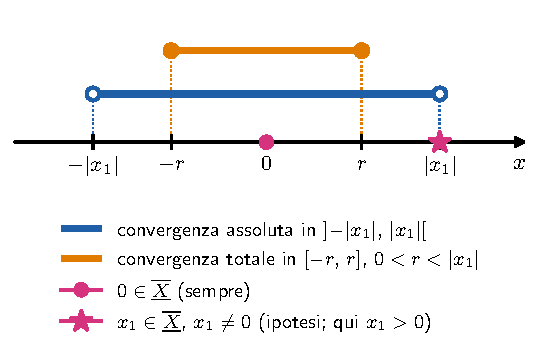
\includegraphics[width=0.8\linewidth]{figure/fig_10}\caption{Teorema~1, parte~1: se la serie converge in $x_1\neq0$ (nel disegno
$x_1>0$), converge assolutamente in $\mathopen{]}-|x_1|,|x_1|\mathclose{[}$ (in
blu) e totalmente in ogni $[-r,r]$ con $0<r<|x_1|$.}\label{fig:10}\end{figure}

\paragraph{Osservazione.}
% [0:32:52]
Per la parte~1 basta \emph{un solo} punto $x_1\neq0$ di convergenza per avere la
convergenza assoluta in tutto l'intervallo simmetrico
$\mathopen{]}-|x_1|,|x_1|\mathclose{[}$; per la convergenza totale bisogna
restringersi un po', a $[-r,r]$, come per la serie geometrica.
% [0:34:30]
Nella parte~2 non serve chiedere $x_2\neq0$: in $0$ la serie converge sempre.
La parte~2 dice che, trovato un punto di non convergenza, la serie non converge
nelle ``code'' $|x|>|x_2|$, cioè lontano da $0$.
% [0:35:48]
In particolare non serve studiare a parte i punti negativi, e $\Xconv$ potrà essere
solo $\{0\}$, un intervallo di centro $0$ oppure tutto $\mathbb{R}$: proprietà
che una serie di funzioni qualsiasi non ha.

% [0:37:02]
\paragraph{Dimostrazione della parte 1.} Sia $x_1\neq0$, $x_1\in \Xconv$: la serie
numerica $\sum_{n=0}^{\infty}a_nx_1^n$ converge.
% [0:38:26]
Deduciamo da questa ipotesi tutto ciò che si può con l'Analisi~1:
\begin{itemize}
  \item il termine generale è infinitesimo (condizione necessaria):
  \[
    a_nx_1^n\to0 ;
  \]
  \item % [0:39:53]
  una successione convergente è limitata, quindi esiste $M>0$ tale che
  \begin{equation}\tag{$*$}
    |a_nx_1^n|\le M\qquad\forall n\in\mathbb{N}.
  \end{equation}
\end{itemize}

\emph{Convergenza assoluta.} Sia $x$ con $0<|x|<|x_1|$ (in $x=0$ la convergenza
è già nota): dimostriamo che converge la serie
\[
  \sum_{n=0}^{\infty}|a_nx^n| .
\]
% [0:42:38]
L'idea è maggiorare con qualcosa che converge, usando l'unica disuguaglianza a
disposizione, $(*)$: moltiplichiamo e dividiamo per $x_1^n$ (lecito perché
$x_1\neq0$) e usiamo il fatto che il modulo del prodotto è il prodotto dei
moduli:
\begin{equation}\tag{$**$}
  |a_nx^n|=\underbrace{|a_nx_1^n|}_{\le M\text{ per }(*)}\cdot\left|\frac{x^n}{x_1^n}\right|
  \le M\left|\frac{x^n}{x_1^n}\right|=M\left(\frac{|x|}{|x_1|}\right)^{n}
  \qquad\forall n .
\end{equation}
Passando alle serie (a termini positivi, quindi il confronto si conserva):
\[
  \sum_{n=0}^{\infty}|a_nx^n|\le M\sum_{n=0}^{\infty}\left(\frac{|x|}{|x_1|}\right)^{n}.
\]
A destra c'è una serie geometrica di ragione $0<|x|/|x_1|<1$, quindi
convergente. Per il criterio del confronto la serie converge assolutamente per
ogni $x$ con $|x|<|x_1|$.
% [0:45:18]
Ecco perché la serie geometrica è stata studiata prima: qui fa da serie di
confronto.

\emph{Convergenza totale.}
% [0:46:44]
Bisogna restringersi ancora, prendendo la $x$ un po' più vicina a $0$. Sia
$0<r<|x_1|$: per $|x|\le r$ si maggiora ulteriormente la catena $(**)$:
\[
  |a_nx^n|\le M\left(\frac{|x|}{|x_1|}\right)^{n}\le M\left(\frac{r}{|x_1|}\right)^{n}=M_n
  \qquad\forall n,\ \forall x\in[-r,r].
\]
$M_n$ non dipende da $x$ e $\sum_{n=0}^{\infty}M_n$ converge, essendo una serie
geometrica di ragione $r/|x_1|<1$: la serie converge totalmente in $[-r,r]$.

\paragraph{Osservazione.}
% [0:46:44]
Perché non maggiorare subito con $|x|\le|x_1|$? Si otterrebbe $M_n=M$, e la
serie $\sum_{n=0}^{\infty}M$ diverge (le somme parziali valgono $M(n+1)$):
nessuna informazione. Serve un $r$ \emph{strettamente} minore di $|x_1|$,
% [0:49:29]
così come per la serie geometrica bisognava restare lontani da $1$.
% [0:50:51]
È il ragionamento fatto per la serie geometrica, ma senza usare somme parziali e
somma: per questo funziona per una serie qualunque.

% [0:52:58]
\paragraph{Dimostrazione della parte 2.} Sia $x_2$ un punto in cui la serie non
converge: dobbiamo dimostrare che non converge in nessun $x$ con $|x|>|x_2|$.
% [0:54:23]
Per assurdo, sia $x$ con $|x|>|x_2|$ e supponiamo che la serie converga in $x$
(figura~\ref{fig:11}). Si ha $x\neq0$, perché $|x|>|x_2|>0$ (infatti
$x_2\neq0$, dato che in $0$ la serie converge). Allora, per la parte~1
(applicata con $x$ al posto di $x_1$), la serie converge in
$\mathopen{]}-|x|,|x|\mathclose{[}$, che contiene $x_2$ perché $|x_2|<|x|$
(figura~\ref{fig:12}). Quindi la serie converge anche in $x_2$, contro
l'ipotesi: assurdo.
% [0:57:50]
Dunque la serie non converge in $x$.

\begin{figure}[htbp]\centering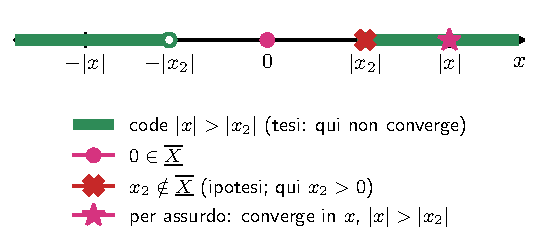
\includegraphics[width=0.8\linewidth]{figure/fig_11}\caption{Teorema~1, parte~2: $x_2$ è un punto di non convergenza (nel disegno
$x_2>0$); per assurdo si suppone che la serie converga in un punto $x$ delle
code $|x|>|x_2|$.}\label{fig:11}\end{figure}

\begin{figure}[htbp]\centering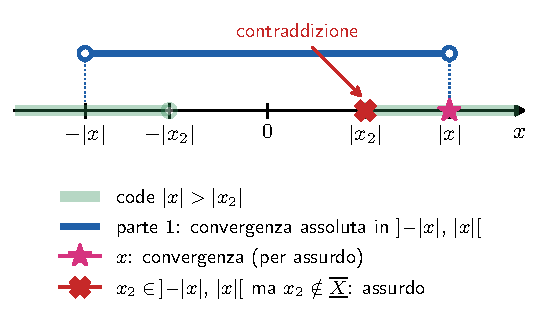
\includegraphics[width=0.8\linewidth]{figure/fig_12}\caption{Conclusione dell'assurdo: per la parte~1 la serie converge in
$\mathopen{]}-|x|,|x|\mathclose{[}$, che contiene il punto di non convergenza
$x_2$.}\label{fig:12}\end{figure}

\paragraph{Osservazione (gli estremi).}
% [0:57:50]
Se la serie converge in $x$ non è detto che converga in $-x$: all'intervallo
$\mathopen{]}-|x|,|x|\mathclose{[}$ si può aggiungere il punto $x$, ma non il
suo simmetrico. Per questo gli intervalli del Teorema~1 sono aperti. Ad esempio
$\sum_{n\ge1}x^n/n$ (vedi l'esempio svolto alla fine) converge in $x=-1$ ma non
in $x=1$: il suo insieme di convergenza è $[-1,1\mathclose{[}$.
% [0:59:19]
Da quale parte si possa chiudere l'intervallo dipende quindi dal segno del
punto, e a priori non si può chiudere.

% [1:00:05]
\subsection{Il raggio di convergenza}

Dal Teorema~1 segue il Teorema~2, che dice com'è fatto il raggio di convergenza
e quindi l'insieme di convergenza.

\paragraph{Teorema 2.} Sia $\sum_{n=0}^{\infty}a_nx^n$ una serie di potenze con
raggio di convergenza $\rho$. Allora:
\begin{enumerate}
  \item $\rho=0$ $\Longleftrightarrow$ la serie converge solo in $x=0$, cioè
  $\Xconv=\{0\}$;
  \item $\rho=+\infty$ $\Longleftrightarrow$ la serie converge assolutamente (e
  puntualmente) in tutto $\mathbb{R}$, cioè $\Xconv=\mathbb{R}$, e totalmente nei
  compatti;
  \item se $0<\rho<+\infty$, la serie converge assolutamente in
  $\mathopen{]}-\rho,\rho\mathclose{[}$, totalmente in $[-r,r]$ per ogni $r$
  con $0<r<\rho$, e non converge per $|x|>\rho$. Quindi
  \[
    \mathopen{]}-\rho,\rho\mathclose{[}\;\subseteq\; \Xconv\;\subseteq\;[-\rho,\rho] .
  \]
\end{enumerate}

\paragraph{Osservazione (il candidato insieme di convergenza).}
% [1:06:45]
Verrebbe da scrivere $\Xconv=\mathopen{]}-\rho,\rho\mathclose{[}$, ma questo è solo
il \emph{candidato} insieme di convergenza: $\rho$ è un sup e non
necessariamente un massimo, quindi a priori non sappiamo se $\pm\rho$ stiano in
$\Xconv$. Le parentesi vanno lasciate aperte, anche se nulla vieta che si chiudano.
Per stabilirlo bisogna studiare la convergenza agli estremi $x=\rho$ e
$x=-\rho$, cioè le due serie numeriche
\[
  \sum_{n=0}^{\infty}a_n\rho^n \qquad\text{e}\qquad \sum_{n=0}^{\infty}(-1)^n a_n\rho^n .
\]
% [1:08:00]
L'esercizio quindi ``raddoppia'': trovato $\rho$ si scrive subito il candidato
per $\Xconv$, ma per sapere se l'intervallo si chiude servono due serie numeriche di
Analisi~1.

\paragraph{Questioni aperte.} Restano due domande:
\begin{enumerate}
  \item come si calcola $\rho$?
  \item se l'insieme di convergenza si chiude in un estremo, cosa si può dire
  della convergenza totale e di quella uniforme?
\end{enumerate}
% [1:09:25]
Alla prima rispondono i criteri seguenti, del tutto meccanici. Alla seconda
risponderà il \emph{teorema di Abel}, che sarà solo enunciato (senza
dimostrazione) e va saputo applicare: se la serie converge in un estremo, la
convergenza uniforme arriva fino a quell'estremo; la totale, in generale, no
(vedi l'esempio svolto).

% [1:12:11]
\subsection{Criterio di Hadamard}

\paragraph{Teorema (criterio di Hadamard).} Sia $\sum_{n=0}^{\infty}a_nx^n$ una
serie di potenze. Se esiste
\[
  \lim_{n\to\infty}\sqrt[n]{|a_n|}=\ell
\]
(per la permanenza del segno $\ell\ge0$), allora
\[
  \rho=\begin{cases}
    0 & \text{se } \ell=+\infty,\\[2pt]
    +\infty & \text{se } \ell=0,\\[2pt]
    \dfrac{1}{\ell} & \text{se } 0<\ell<+\infty.
  \end{cases}
\]
Per l'algebra dei limiti (con $1/(+\infty)=0$ e $1/0^+=+\infty$) si può scrivere
in un'unica formula
\[
  \rho=\frac{1}{\ell}.
\]

\paragraph{Richiamo (criterio della radice per le serie numeriche).} Sia
$b_n\ge0$ e sia $\lim_{n\to\infty}\sqrt[n]{b_n}=\ell$. Allora:
\begin{itemize}
  \item se $\ell>1$ (anche $\ell=+\infty$), si ha $b_n>1$ definitivamente,
  quindi $b_n\not\to0$ e $\sum b_n=+\infty$;
  \item se $0\le\ell<1$, $\sum b_n$ converge;
  \item se $\ell=1$ il criterio non è conclusivo.
\end{itemize}

\paragraph{Dimostrazione.}
% [1:16:55]
Si procede come nello studio di una qualunque serie di funzioni: per ogni $x$
fissato si applicano i criteri dell'Analisi~1. È l'esercizio che si farebbe su
una serie assegnata senza conoscere il teorema; sistematizzato, diventa un
criterio. La serie non ha segno costante (la $x$ varia in tutto $\mathbb{R}$),
quindi si studia la convergenza assoluta, cioè la serie
$\sum_{n=0}^{\infty}|a_nx^n|$, con il criterio della radice (non con quello di
Hadamard, che è ciò che si sta dimostrando).
% [1:17:54]
Per $x\neq0$ (in $x=0$ c'è sempre convergenza; per $\ell=+\infty$ si avrebbe
anche la forma indeterminata $\infty\cdot0$)
\[
  \lim_{n\to\infty}\sqrt[n]{|a_nx^n|}
  =\underbrace{\lim_{n\to\infty}\sqrt[n]{|a_n|}}_{=\,\ell\text{ per ipotesi}}\cdot|x|
  =\ell\,|x| ,
\]
% [1:19:16]
perché $|x|$ non dipende da $n$ ed esce dal limite (il modulo va messo su tutto,
anche su $a_n$). Per il richiamo:
\begin{itemize}
  \item se $\ell|x|<1$, la serie converge assolutamente in $x$;
  \item se $\ell|x|>1$, allora $|a_nx^n|>1$ definitivamente: il termine
  generale non è infinitesimo e la serie \emph{non converge} in $x$ (non solo
  non converge assolutamente).\footnote{Questo passaggio non è stato esplicitato
  a lezione, dove si è mostrata solo la convergenza per $\ell|x|<1$. Senza di
  esso si otterrebbe solo $\rho\ge1/\ell$.}
\end{itemize}
% [1:20:33]
Distinguiamo i casi su $\ell$:
\begin{itemize}
  \item $\ell=+\infty$: $\ell|x|=+\infty>1$ per ogni $x\neq0$, quindi la serie
  converge solo in $0$ e $\rho=0$;
  \item $\ell=0$: $\ell|x|=0<1$ per ogni $x$, quindi la serie converge in tutto
  $\mathbb{R}$ e $\rho=+\infty$;
  \item % [1:22:02]
  $0<\ell<+\infty$: la serie converge per $|x|<1/\ell$ e non converge per
  $|x|>1/\ell$, cioè
  \[
    \mathopen{]}-\tfrac1\ell,\tfrac1\ell\mathclose{[}\;\subseteq\; \Xconv\;\subseteq\;
    \bigl[-\tfrac1\ell,\tfrac1\ell\bigr]
    \qquad\Longrightarrow\qquad \rho=\frac{1}{\ell}.
  \]
\end{itemize}
Per $|x|=1/\ell$ si ha $\ell|x|=1$ e il criterio della radice non decide: è per
questo che gli estremi vanno studiati a parte.

% [1:23:12]
\subsection{Criterio di D'Alembert}

Dal criterio rapporto-radice dell'Analisi~1 segue un altro criterio, che si
deve a d'Alembert (equivalente al precedente quando il limite del rapporto
esiste).

\paragraph{Teorema (criterio di D'Alembert).} Sia $\sum_{n=0}^{\infty}a_nx^n$
una serie di potenze con $a_n\neq0$ definitivamente. Se esiste
\[
  \lim_{n\to\infty}\left|\frac{a_{n+1}}{a_n}\right|=\ell ,
\]
allora $\rho=1/\ell$, con la stessa convenzione del criterio di Hadamard
($\rho=+\infty$ se $\ell=0$, $\rho=0$ se $\ell=+\infty$).

\paragraph{Dimostrazione.}
% [1:25:20]
Per il criterio rapporto-radice per le successioni, se il limite del rapporto
vale $\ell$, anche il limite della radice $n$-esima vale $\ell$:
\[
  \lim_{n\to\infty}\left|\frac{a_{n+1}}{a_n}\right|=\ell
  \quad\Longrightarrow\quad
  \lim_{n\to\infty}\sqrt[n]{|a_n|}=\ell ,
\]
quindi vale la tesi del criterio di Hadamard.

\paragraph{Osservazione (non dimenticare i moduli).} In entrambi i criteri il
modulo serve ad avere termini positivi, e solo in quel caso si possono
applicare i criteri della radice e del rapporto.
% [1:25:20]
Dimenticarlo non è un errore da poco: il limite potrebbe venire negativo, cosa
impossibile per un raggio.

\paragraph{Osservazione (radice o rapporto).} Il criterio della radice è più
generale: se esiste il limite del rapporto esiste anche quello della radice, ma
non viceversa. Ad esempio con
\[
  a_n=\begin{cases}1 & n\ \text{pari}\\ 2 & n\ \text{dispari}\end{cases}
  \qquad\Longrightarrow\qquad
  \left|\frac{a_{n+1}}{a_n}\right|\in\Bigl\{2,\frac12\Bigr\},
  \qquad \sqrt[n]{|a_n|}\to1
\]
il rapporto non ha limite, mentre Hadamard dà $\rho=1$. Inoltre D'Alembert non
si applica se infiniti coefficienti sono nulli: nella serie del seno, ad
esempio, compaiono solo le potenze dispari; Hadamard invece funziona
($\sqrt[n]{|a_n|}\to0$, quindi $\rho=+\infty$).
% [1:26:48]
Se non esiste nemmeno il limite della radice si usa la formula di
Cauchy--Hadamard, che vale sempre:
\[
  \frac{1}{\rho}=\limsup_{n\to\infty}\sqrt[n]{|a_n|}.
\]
Il $\limsup$ va preso sulla radice, non sul rapporto: nell'esempio sopra il
$\limsup$ del rapporto vale $2$ e darebbe $\rho=1/2$, che è sbagliato.
Calcolare $\rho$ non è quindi il vero problema: la parte delicata è capire cosa
succede agli estremi.

% [1:14:20]
\subsection{Esempio svolto}

\paragraph{Esempio.} Studiamo la serie
\[
  \sum_{n=1}^{\infty}\frac{x^n}{n}.
\]
% [1:14:20]
Prima di tutto si riconosce che è una serie di potenze: la potenza è $x^n$ e il
coefficiente è $a_n=1/n$ (la somma parte da $n=1$: manca il termine noto, cioè
$a_0=0$). Con il criterio di Hadamard:
\[
  \frac{1}{\rho}=\ell=\lim_{n\to\infty}\sqrt[n]{\left|\frac{1}{n}\right|}
  =\lim_{n\to\infty}\frac{1}{\sqrt[n]{n}}=1
  \qquad\Longrightarrow\qquad \rho=1 .
\]
Il candidato insieme di convergenza è quindi $\mathopen{]}-1,1\mathclose{[}$, in
cui la serie converge assolutamente.
% [1:15:39]
L'esercizio si riduce a un limite di successione (niente condizione necessaria
né il resto dello studio di una serie): bisogna ricordare bene i limiti di
successione.

Restano gli estremi:
\begin{itemize}
  \item $x=1$: si ottiene $\displaystyle\sum_{n=1}^{\infty}\frac{1}{n}$, la serie
  armonica, che diverge;
  \item $x=-1$: si ottiene $\displaystyle\sum_{n=1}^{\infty}\frac{(-1)^n}{n}$, la
  serie armonica a segni alterni, che converge.
\end{itemize}
Quindi
\[
  \Xconv=[-1,1\mathclose{[} .
\]
Fino all'estremo chiuso la convergenza totale non arriva: in $[-1,0]$
\[
  \sup_{x\in[-1,0]}\left|\frac{x^n}{n}\right|=\frac{1}{n}
  \qquad\text{e}\qquad \sum_{n=1}^{\infty}\frac{1}{n}=+\infty .
\]
Che arrivi almeno la convergenza uniforme lo dirà il teorema di Abel.

\paragraph{Osservazione (serie di potenze e Taylor).}
% [1:28:15]
Tutto questo non è astratto, anzi. Con i coefficienti di Taylor visti
all'inizio, il polinomio di Taylor diventa una serie (per il seno compaiono solo
le potenze dispari). Dove si dimostra che una funzione è la somma della sua
serie di Taylor, la funzione è davvero un ``polinomio infinito'', e si capisce
perché la si scriveva come il suo polinomio di Taylor ``a meno di un errore'':
al crescere del grado i polinomi di Taylor del seno approssimano il seno su
intervalli sempre più grandi, ma per avere tutto il seno serve la somma
infinita.
% [1:29:38]
La teoria delle serie di potenze spiega perché Taylor funziona. Non è però
automatico: $\ln(1+x)$ coincide con la sua serie di Taylor solo in
$\mathopen{]}-1,1]$, e la funzione $e^{-1/x^2}$ (posta uguale a $0$ in $0$) ha
serie di Taylor in $0$ identicamente nulla, pur non essendo nulla.
